\documentclass[11pt,a4paper]{article}
\usepackage[margin=18mm]{geometry}
\usepackage{amsmath,amssymb,mathtools}
\usepackage{booktabs,array,enumitem}
\usepackage[dvipsnames]{xcolor}
\usepackage{listings}
\usepackage{tikz}
\usetikzlibrary{arrows.meta,positioning}
\usepackage[most]{tcolorbox}
\usepackage{hyperref}
\hypersetup{colorlinks=true,urlcolor=MidnightBlue,linkcolor=MidnightBlue}
\setlength{\parindent}{0pt}
\setlength{\parskip}{4pt}
\newcommand{\course}{Computational Methods in Physics}
\newtcolorbox{keybox}{colback=RoyalBlue!5,colframe=RoyalBlue!65!black,boxrule=.7pt,arc=2mm}
\newtcolorbox{checkbox}{colback=ForestGreen!5,colframe=ForestGreen!55!black,boxrule=.7pt,arc=2mm}
\newtcolorbox{aibox}{colback=BurntOrange!7,colframe=BurntOrange!80!black,boxrule=.7pt,arc=2mm}
\lstdefinestyle{matlabstyle}{
  language=Matlab,
  basicstyle=\ttfamily\footnotesize,
  keywordstyle=\color{RoyalBlue!75!black},
  commentstyle=\color{ForestGreen!55!black},
  stringstyle=\color{BurntOrange!80!black},
  numbers=left,
  numberstyle=\scriptsize\color{black!50},
  numbersep=5pt,
  frame=single,
  rulecolor=\color{RoyalBlue!25},
  backgroundcolor=\color{RoyalBlue!3},
  showstringspaces=false,
  columns=fullflexible,
  keepspaces=true,
  breaklines=true
}
\begin{document}

{\large\textsc{\course}}\\[-2pt]
{\small Learning Note \textbar\ Week 2}\par\vspace{4pt}
{\LARGE\bfseries Reliable Computational Workflow Through Physics}\par\vspace{3pt}
\textit{Reliable code makes the physical dependencies and the evidence for trust visible.}

\begin{keybox}
\textbf{Physical question.} Can we construct an ideal mass-spring oscillator calculation that is readable, testable, and capable of exposing a plausible but physically wrong result?
\end{keybox}

\section*{Learning outcomes}
By the end of this week, you should be able to:
\begin{enumerate}[nosep,leftmargin=5mm]
  \item decompose a physics question into inputs, derived quantities, outputs, and checks;
  \item express dependencies as structured pseudocode before implementation;
  \item use vectorised MATLAB expressions while preserving units and array shapes;
  \item distinguish syntax, logical, numerical, and physical defects; and
  \item design several independent tests and explain what each test can detect.
\end{enumerate}

\section*{1. A computational result is an argument}
A program is not trustworthy merely because it runs. It makes a chain of claims: the model represents the intended physics, quantities have consistent units, the algorithm follows the model, arrays align, and the output satisfies independent expectations.

\begin{center}
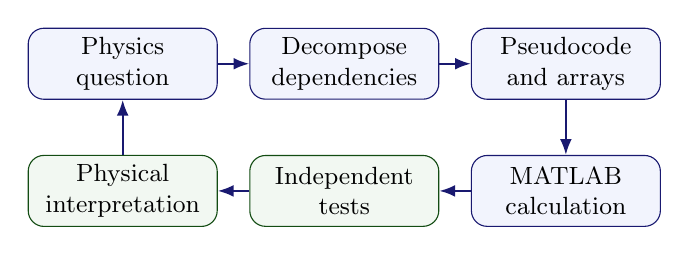
\begin{tikzpicture}[node distance=7mm and 4mm,every node/.style={font=\small,align=center},box/.style={draw=MidnightBlue,rounded corners=2mm,fill=RoyalBlue!7,minimum width=24mm,minimum height=9mm},test/.style={draw=ForestGreen!55!black,rounded corners=2mm,fill=ForestGreen!6,minimum width=24mm,minimum height=9mm},arrow/.style={-{Latex[length=2mm]},thick,MidnightBlue}]
\node[box] (q) {Physics\\question};
\node[box,right=of q] (d) {Decompose\\dependencies};
\node[box,right=of d] (p) {Pseudocode\\and arrays};
\node[box,below=of p] (c) {MATLAB\\calculation};
\node[test,left=of c] (t) {Independent\\tests};
\node[test,left=of t] (i) {Physical\\interpretation};
\draw[arrow] (q)--(d); \draw[arrow] (d)--(p); \draw[arrow] (p)--(c);
\draw[arrow] (c)--(t); \draw[arrow] (t)--(i); \draw[arrow] (i)--(q);
\end{tikzpicture}
\end{center}

When a test fails, treat debugging as another controlled experiment. Change one suspected cause and observe whether the predicted symptom changes.

\section*{2. Worked model: an ideal mass-spring oscillator}
For a horizontal oscillator with mass $m$, spring constant $k$, and displacement $x$ from equilibrium,
\begin{equation}
  m\frac{d^2x}{dt^2}=-kx.
\end{equation}
For amplitude $A$ and phase $\phi$, the analytical position and velocity are
\begin{align}
  x(t)&=A\cos(\omega t+\phi),\\
  v(t)&=-A\omega\sin(\omega t+\phi),\\
  \omega&=\sqrt{\frac{k}{m}}, \qquad T=\frac{2\pi}{\omega}.
\end{align}
The ideal model assumes a linear spring, constant mass, one-dimensional motion, no damping, and equilibrium at $x=0$.

For $m=0.50\,\mathrm{kg}$ and $k=8.0\,\mathrm{N\,m^{-1}}$, $\omega=4.0\,\mathrm{rad\,s^{-1}}$ and $T=\pi/2\,\mathrm{s}$. If the mass is released from rest at $x=A=0.12\,\mathrm{m}$, then $\phi=0$.

\begin{checkbox}
\textbf{Predict before computing.}
\begin{itemize}[nosep,leftmargin=5mm]
  \item At $t=T/4$, should the velocity be positive or negative?
  \item What are the allowed bounds on $x$?
  \item How should kinetic, potential, and total energy behave?
\end{itemize}
\end{checkbox}

\section*{3. Decompose before writing MATLAB}
Separate four kinds of information:
\begin{center}
\small
\begin{tabular}{>{\raggedright\arraybackslash}p{.20\linewidth}>{\raggedright\arraybackslash}p{.68\linewidth}}
\toprule
\textbf{Layer} & \textbf{Oscillator example}\\ \midrule
Inputs & $m$, $k$, $A$, $\phi$, final time, and sampling resolution\\
Derived quantities & $\omega=\sqrt{k/m}$ and $T=2\pi/\omega$\\
Outputs & $x(t)$, $v(t)$, kinetic energy, potential energy, and total energy\\
Checks & initial state, displacement bounds, one-period repeat, energy conservation, and the predicted velocity sign\\ \bottomrule
\end{tabular}
\end{center}

Pseudocode should preserve this dependency order:
\begin{enumerate}[nosep,leftmargin=6mm]
  \item Define physical inputs with units.
  \item Compute $\omega$ and $T$.
  \item Create one time array.
  \item Evaluate $x$, $v$, $K$, $U$, and $E$ at the same times.
  \item Apply independent checks.
  \item Interpret the motion and state the model limitations.
\end{enumerate}

Pseudocode is not an informal decoration. It is an explicit description of which quantities depend on which earlier decisions.

\section*{4. Vectorisation and array-shape contracts}
MATLAB evaluates the analytical model for all times using arrays:
\begin{lstlisting}[style=matlabstyle,caption={Vectorised oscillator calculation}]
mass_kg = 0.50;
springConstant_N_per_m = 8.0;
amplitude_m = 0.12;
omega_rad_per_s = sqrt(springConstant_N_per_m/mass_kg);
period_s = 2*pi/omega_rad_per_s;

t_s = linspace(0,4*period_s,1001);
x_m = amplitude_m.*cos(omega_rad_per_s.*t_s);
v_m_per_s = -amplitude_m.*omega_rad_per_s.*sin(omega_rad_per_s.*t_s);
K_J = 0.5*mass_kg.*v_m_per_s.^2;
U_J = 0.5*springConstant_N_per_m.*x_m.^2;
E_J = K_J + U_J;
\end{lstlisting}

The operator \texttt{.\^{}2} squares every stored value. The arrays \texttt{t\_s}, \texttt{x\_m}, \texttt{v\_m\_per\_s}, and \texttt{E\_J} must have the same shape. Treat this as an interface contract:
\begin{lstlisting}[style=matlabstyle]
assert(isequal(size(t_s),size(x_m),size(v_m_per_s),size(E_J)), ...
    'The computed arrays do not share one aligned shape.')
\end{lstlisting}

Vectorisation is not automatically better physics. It is a compact way to apply the same independent calculation to aligned inputs. A scalar loop that evaluates the same formula should agree to round-off precision.

\section*{5. Layer tests that can fail independently}
Testing should move from basic execution toward physical meaning.
\begin{center}
\small
\begin{tabular}{>{\raggedright\arraybackslash}p{.23\linewidth}>{\raggedright\arraybackslash}p{.43\linewidth}>{\raggedright\arraybackslash}p{.23\linewidth}}
\toprule
\textbf{Test layer} & \textbf{Example} & \textbf{What it can expose}\\ \midrule
Shape and finiteness & All arrays align and contain finite values & indexing and array-operation defects\\
Known value & $x(0)=A$, $v(0)=0$ & initial-condition and phase defects\\
Physical bound & $|x|\le A$ & scaling or formula defects\\
Repeat case & $x(T)=x(0)$ & period and frequency defects\\
Invariant & $K+U=\tfrac12 kA^2$ & inconsistent position, velocity, or energy formulas\\
Phase prediction & $v(T/4)<0$ & a velocity-sign defect that energy alone misses\\ \bottomrule
\end{tabular}
\end{center}

The total energy is
\begin{equation}
 E(t)=\frac12mv^2+\frac12kx^2=\frac12kA^2.
\end{equation}
A missing minus sign in $v(t)$ does not change $v^2$. Therefore, incorrect velocity can still pass the energy test. This is why several tests with different failure sensitivities are stronger than one impressive invariant.

\begin{aibox}
\textbf{Caution: a passing test is evidence, not proof.} State what the test was designed to detect and identify at least one plausible error it would not detect.
\end{aibox}

\section*{6. Diagnose defects by category}
Different defects require different evidence:
\begin{center}
\small
\begin{tabular}{>{\raggedright\arraybackslash}p{.20\linewidth}>{\raggedright\arraybackslash}p{.34\linewidth}>{\raggedright\arraybackslash}p{.35\linewidth}}
\toprule
\textbf{Category} & \textbf{Example} & \textbf{Useful first test}\\ \midrule
Syntax & unmatched bracket or invalid operator & reproduce the exact MATLAB message\\
Logical & \texttt{0:tMax:dt} reverses the colon arguments & inspect endpoints and number of values\\
Array & \texttt{v\^{}2} uses matrix power for a vector & inspect shape; replace with \texttt{v.\^{}2}\\
Numerical & exact equality is used for a sampled threshold & vary resolution or use a tolerance\\
Physical & $\omega=\sqrt{km}$ instead of $\sqrt{k/m}$ & check dimensions and period scale\\
Communication & axes are reversed or unlabelled & another reader cannot interpret the output\\ \bottomrule
\end{tabular}
\end{center}

Use a controlled debugging cycle:
\begin{enumerate}[nosep,leftmargin=6mm]
  \item reproduce the symptom from a clean run;
  \item localise the first doubtful quantity;
  \item state one hypothesis about the cause;
  \item design the smallest test that distinguishes that hypothesis;
  \item repair one cause and rerun all tests; and
  \item explain the physical consequence of the defect.
\end{enumerate}

\section*{7. Reading plausible AI-generated code}
Consider this candidate:
\begin{lstlisting}[style=matlabstyle]
omega_rad_per_s = sqrt(springConstant_N_per_m*mass_kg);
t_s = 0:4*period_s:0.01;
x_m = amplitude_m*cos(omega_rad_per_s*t_s);
energy_J = 0.5*mass_kg*v_m_per_s^2 ...
         + 0.5*springConstant_N_per_m*x_m^2;
plot(x_m,t_s)
\end{lstlisting}

It contains a physical/formula defect, a logical time-array defect, array-power defects, and a communication defect. Do not ask only ``Will MATLAB run this?'' Ask what each line claims, which consequence follows, and which independent test would fail.

\begin{aibox}
\textbf{Responsible AI use.} Record what Copilot was asked to do, what was accepted, modified, or rejected, why that decision was made, and which independent checks were performed. A confident explanation from AI is not validation evidence.
\end{aibox}

\section*{8. Practical transfer: projectile motion}
The practical transfers the workflow to a projectile launched from height $y_0$ with speed $v_0$ and angle $\theta$:
\begin{align}
 x(t)&=v_0\cos\theta\,t,\\
 y(t)&=y_0+v_0\sin\theta\,t-\frac12gt^2.
\end{align}
The model assumes uniform gravity, negligible air resistance, a point-like projectile, and level ground at $y=0$.

For $v_0=18.0\,\mathrm{m\,s^{-1}}$, $\theta=40^\circ$, and $y_0=1.5\,\mathrm{m}$, useful references are:
\begin{center}
\small
\begin{tabular}{lr}
\toprule
\textbf{Quantity} & \textbf{Reference value}\\ \midrule
Horizontal speed & $13.7888\,\mathrm{m\,s^{-1}}$\\
Initial vertical speed & $11.5702\,\mathrm{m\,s^{-1}}$\\
Flight time & $2.48206\,\mathrm{s}$\\
Horizontal range & $34.2247\,\mathrm{m}$\\
Peak time & $1.17943\,\mathrm{s}$\\
Peak height & $8.32309\,\mathrm{m}$\\ \bottomrule
\end{tabular}
\end{center}

Strong validation evidence includes the initial position, constant horizontal velocity, the sign change of vertical velocity at the peak, the final ground condition, a reference range, aligned arrays, and finite values.

\section*{Three takeaways}
\begin{enumerate}[nosep,leftmargin=6mm]
  \item Decomposition and pseudocode make the reasoning visible before MATLAB syntax enters.
  \item Vectorisation is reliable only when units, dependencies, and array shapes remain explicit.
  \item Several independent tests are needed because one plausible error may pass one strong-looking check.
\end{enumerate}

\begin{keybox}
\textbf{Preparation for the practical.} Complete the Week 02 Individual Practical Check --- Quiz in Google Classroom first. Then bring the projectile model from physical assumptions to pseudocode, repair the supplied candidate, and defend the validation evidence. MATLAB Copilot is allowed only during group work and every material suggestion must be declared and tested.
\end{keybox}

\end{document}
